\section{Detector models}\label{sec:hist:detect}

One of the considerations we can gather from the previous Sections
is that 
the problem of arrival time ---of a particle at a particular region of space---
can be tackled at differemt ``levels''. 

Operationally, there must be a detector which
``clicks'' at the arrival of the particle, and the statistical distribution of
such click times over repeated measurements is studied. Due the Pauli objection,
probabilities in this distribution cannot simply be given in terms of projectors related to eigenspaces of a self-adjoint operator.
A more general formulation than projective measurement is therefore necessary.

Detectors can be treated more or less explicitly in quantum models of arrival time:
\begin{enumerate}
  \item
    Without making the detector explicit. This is the case of the Kijowski model (Sec. \ref{sec:kijowski}),
    which is based on positive-operator measurement\linebreak(POVM). Given there's no detector in the model,
    the best candidate statistical distribution and operator are essentially obtained
    through consistency arguments including a reasonable classical limit.
  \item
    Early attempts at incorporating the measurement apparatus
    (namely Allcock, Sec. \ref{sec:allcock}) which
    focus on the irreversible process of absoption.
    Normalization of the quantum state is not preserved, the Hamiltonian is not\linebreak{Hermitian}
    because the potential is not real. The rate of normalization-loss is interpreted as
    absorption (detection, arrival) probability over time. The detector is in fact
    ``traced out'' and the particle is treated as an open system (Sec. \ref{sec:halliwell}).
  \item
    Full detector models. For example the Atom-Laser one. Two-level atoms in the ground state
    are sent to a laser-illuminated region (we're interested in the time-of-arrival into this region),
    get excited, and the first photon which is spontaneously emitted following the excitation
    is interpreted as detection of the arrival in the region. Problems related to
    reflection, low absorption rate, and delay in the spontaneous emission are fully taken into account in the model.
\end{enumerate}

A brief, mostly qualitative, illustration of the Atom-Laser model is
given below, and references therein can be consulted for more details.

\subsection{Basics of Atom-Laser Model}

As pointed out in \cite{Damborenea}, the model by Halliwell (Sec. \ref{sec:halliwell})
has the merit of including irreversibility in the detection process,
but ``remains somewhat abstract
since no connection is made with any specific measuring
system''. The work by Damborenea et al. \parencite{Damborenea} gives instead an operational
description of the notion of \emph{arrival time}.

In its essence, the model describes an atom sent toward a laser-illuminated region,
and the arrival time into the region is taken as the time\footnote{
  Please note, while there is an operational definition of detection,
  there is no operational definition of time, in other words,
  while this model does include an explicit description of the detector,
  there is still no description or definition of a ``clock'',
  which is still somewhat implicitly assumed as a ``classical'' one.
  This further motivates theories modelling quantum clocks instead,
  as seen from Chapter \ref{ch:pw} on.
}
when the first photon is spontaneously emitted by the atom,
following its excitation by the laser.
The spontaneous photon emission is therefore the ``click'' of the detector.

This time-of-arrival formulation has been shown in excellent numerical agreement
with Kijowskii axiomatic distribution.

One limitation of the model is given by delays:
\begin{enumerate*}[label=\arabic*)]
  \item in the transition of the atom to the excited state, and
  \item in the spontaneous emission.
\end{enumerate*}
This cannot be addressed by simply increasing the laser intensity
(therefore shortening the excitation and decay time)
because this would lead to elastic reflection,
and the most likely outcome would be no detection/absorption at all.
This is similar to the issue encountered, at a teorethical level,
by Allcock when the imaginary absorbing potential was too large.

A suitable detector configuration, therefore, will be based on \emph{weak driving},
but will need to have the delays compensated,
which can be achieved
by computing the
deconvolution with the decay time distribution of an atom at rest.

The weak driving regime is characterized by longer lifetimes.
However, the paper shows that,
as a limit for shorter lifetimes,
the deconvoluted distribution converges
to
the probability current flux.
This is interesting because, on the other hand, in general,
the probability current cannot be used to derive a time of arrival
distribution, due to the backflow effect
---for instance in a one dimensional system, a superposition of only positive momentum eigenfunctions may still lead to a
negative current, as it was initially noted by Allcock himself \parencite{Allcock-3}.

A possible experimental implementation is actually based on a \emph{3-level} atom,
which decades into an intermediate, metastable, 
``sink'' state after emission so TODO TODO 
that the atom can't be excited again: this motivates studying 3-level systems with PW later; see \cite{Metastable}.

* eq. 4.7 in book, brief mention on how the simplification is obtainied, detuning, on-resonance, so Delta is zero.

* a particular case of it goes on next section (where Kiukas et al heavily cited)

* what params makes little reflection but good prob. of detection?

* fig. 4.3 in book, discrete points, delay (convolution etc.), sec. 4.2.2 book

* in next section we don't care of delay because we study the time of decay rather than the time of arrival of the atom (or we assume they coincide because convolution technique was used).

* $\Pi$ is loss of normalization

\subsection{Ruschhaupt, Kiukas et al}\label{sec:hist:detect:kiukas}

Studies
about detector models which investigate
time-of-arrival as a quantum observable.
In particular we consider \cite{RuschhauptAbsorption},
which in turn traces back its basic ideas from the seminal work by Allcock
in the 1960s \parencite{Allcock-1, Allcock-2, Allcock-3},
while a detailed contemporary formulation can be found in
\cite[Ch. 4]{TQM2}.

A non hermitian Hamiltonian is justified as a computation method
to simplify the study of some open systems: the evolution of mixed
states is derived without explicit reference to density operators
or master equations, but resolving equations that are formally
identical to those of pure states,
i.e. in terms of
Schr{\"o}dinger equations and wave functions,
with the non-hermitian term in the Hamiltonian
to account for the non-unitarity of the evolution.

The detection-by-absoption model in \cite{RuschhauptAbsorption}
is based on a complex potential that, plugged into the Schr\"odinger equation,
leads to a non-unitary evolution of the state vector
(with loss of normalization).

Specifically, the Hamiltonian $\hat{H}$ is replaced by a $\hat{H} - i\hat{D}$
(with $\hat{D}$ self-adjoint, bounded, positive)
and, consequently:
\begin{equation}\label{eq:schrod_complex_pot}
  \hat{H} \ket{\psi(t)} = i\hbar\dv{t}\ket{\psi(t)} +i\hat{D}\ket{\psi(t)} \text{.}
\end{equation}

\citereset\subsection{Application: two-level system}

In \cite{RuschhauptAbsorption}, an example application of the detector model
is provided for a two-level system.
In Page and Wootters terms,
this would corrspond to a bi-dimensional $\hilb{H}_S$, but a continuous
spectrum of $\hat{T}$ in $\hilb{H}_T$. The paper is \emph{not} based on
the Page--Wootters model, indeed the purpose of this section is a comparison
with such model, using the results of Section \ref{sec:absorption+pw}.

By setting, out of convenience, $\hbar = \omega = 1$
(with $\omega$ the characteristic frequency of the system),
and directly considering the parameters
that minimize the time--energy uncertainty product \parencite{RuschhauptAbsorption},
we have a non-Hermitian ``Hamiltonian''
$\mathit{K} = \hat{H} - i\hat{D}$ with
\begin{equation}\label{eq:complexpot}
  \mathit{K} = \hat{H} - i\hat{D} \repr
    \hbar\omega\left\{
      \left[\begin{matrix}0 & 1\\1 & 0\end{matrix}\right] -
      i \left[\begin{matrix}0 & 0\\0 & \gamma \end{matrix}\right]
    \right\}
\end{equation}
and $\gamma = 2\sqrt{2}$.

We take an initial state of $\ket{0}$
(or $\mqty[1\\0]$ in matrix form).

We then compute, symbolically, the non-unitary evolution
$\ket{\psi(t)} = e^{-i\mathit{K}t}\ket{0}$
with the aid of \term{SymPy} \parencite{comp:sympy} within a \term{Jupyter} \parencite{comp:jupyter} notebook
(see Appendix \ref{detector-model-kiukas-ruschhaupt-schmidt-werner} for all the details of the calculation).

Simplifying the result in eq. \eqref{eq:sympy:non-unitary-evol}, we have:
\begin{equation}
  \ket{\psi(t)} \repr e^{-\frac{\sqrt{2}}{t}} \mqty[
    \cos(\frac{\sqrt{2}}{2}t) + \sin(\frac{\sqrt{2}}{2}t)& \\
                     -i\sqrt{2} \sin(\frac{\sqrt{2}}{2}t)&
  ] \,\text{.}
\end{equation}

\begin{figure} %% https://tex.stackexchange.com/a/165730
  \centering
  \begin{subfigure}{0.49\textwidth}
    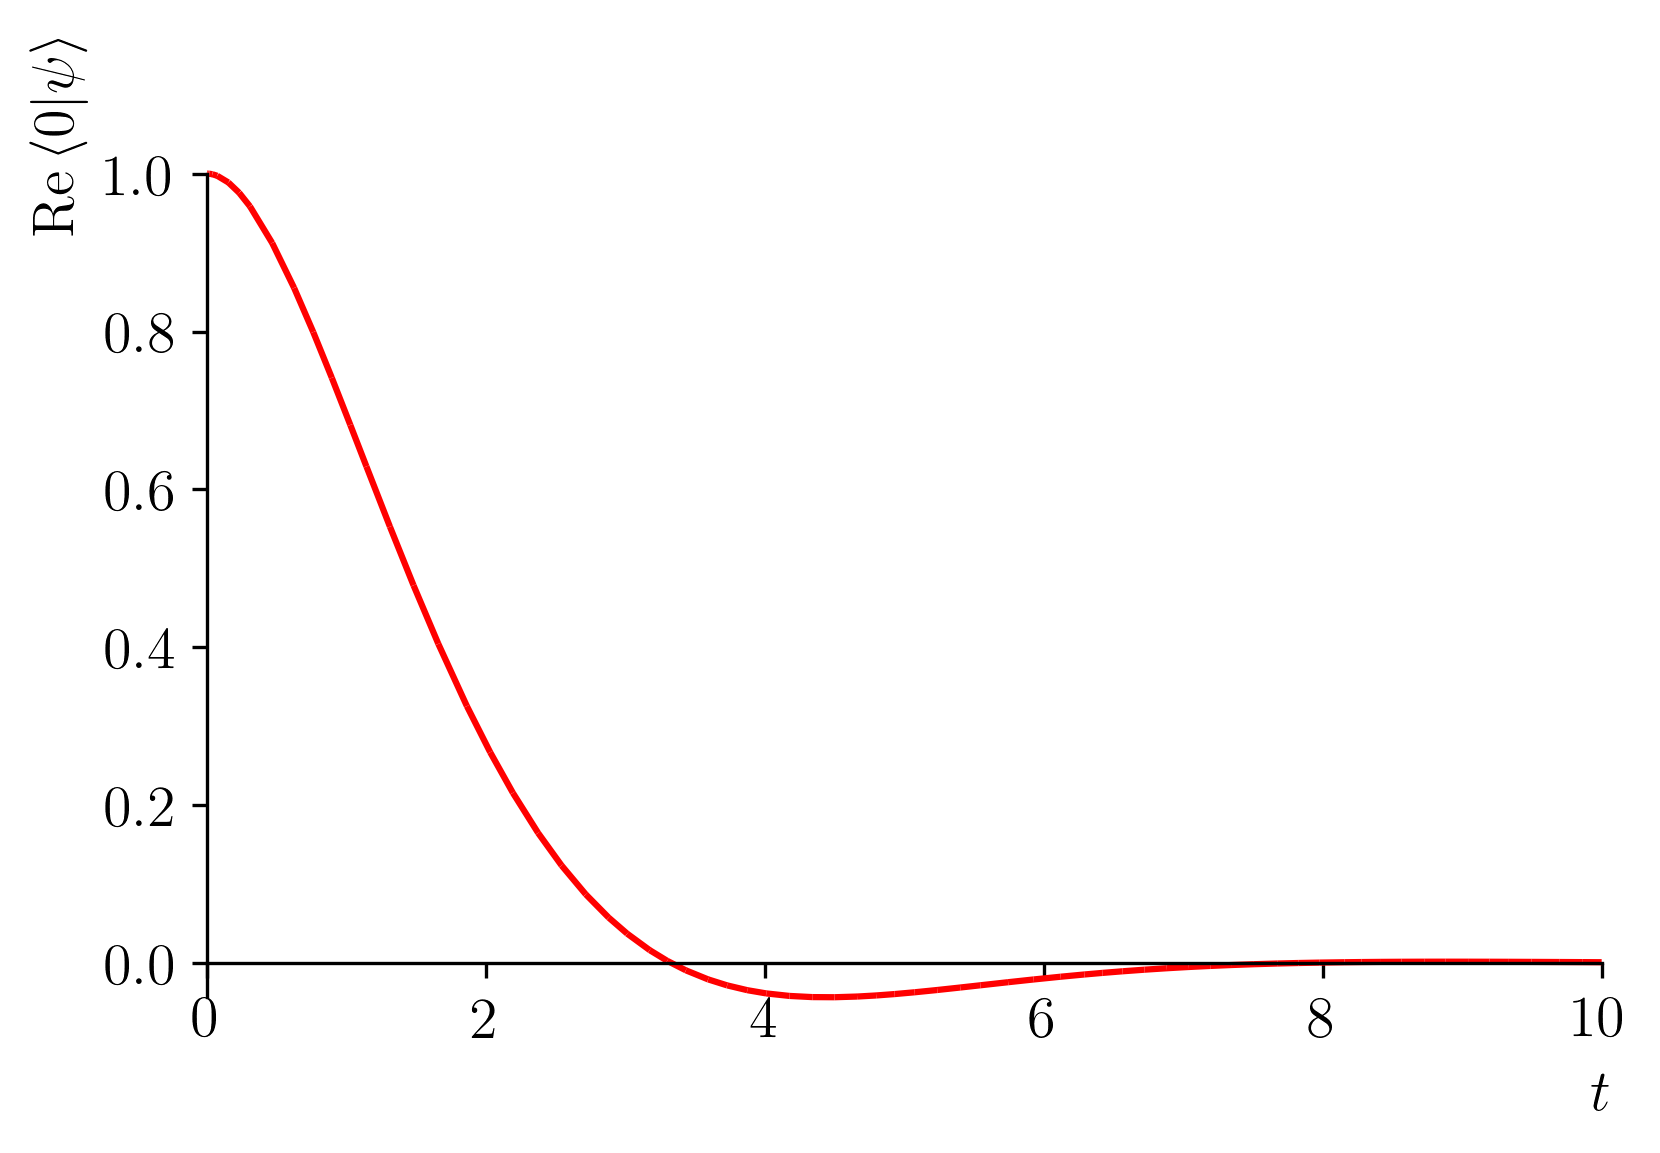
\includegraphics[width=\linewidth]{img/2ldetect/re_psi0_t.png}
    \subcaption{}\label{fig:absorbed-qubit-components:re0}
  \end{subfigure}
  % \hspace*{\fill} % separation between the subfigures
  \begin{subfigure}{0.49\textwidth}
    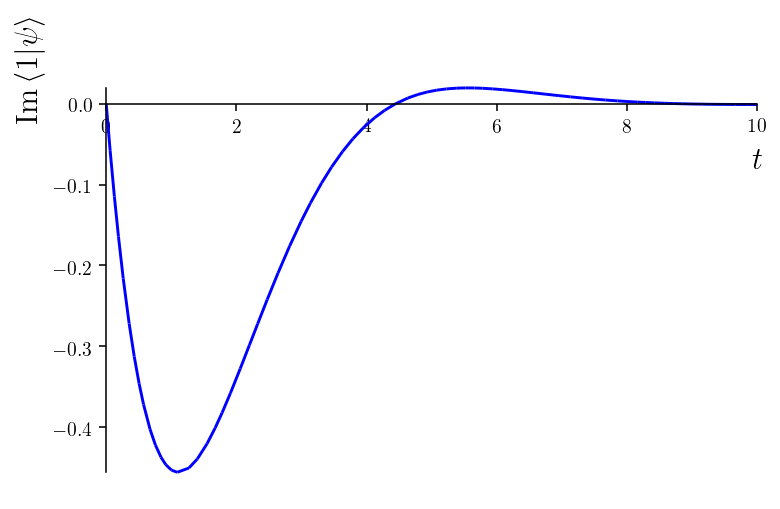
\includegraphics[width=\linewidth]{img/2ldetect/im_psi1_t.png}
    \subcaption{}\label{fig:absorbed-qubit-components:im1}
  \end{subfigure}
  % \hspace*{\fill} % separation between the subfigures
  \caption{
    Non-unitary evolution of the absorbed qubit
    according to the model in
    ref. \cite[sec.``Emission from a two-level system'']{RuschhauptAbsorption}.
    The component along $\ket{0}$ is purely real,
    and the one along $\ket{1}$ is purely imaginary,
    therefore only their their respective parts are plotted.
  }\label{fig:absorbed-qubit-components}
\end{figure}

\begin{figure}
  \centering
  \begin{subfigure}[b]{0.49\textwidth}
    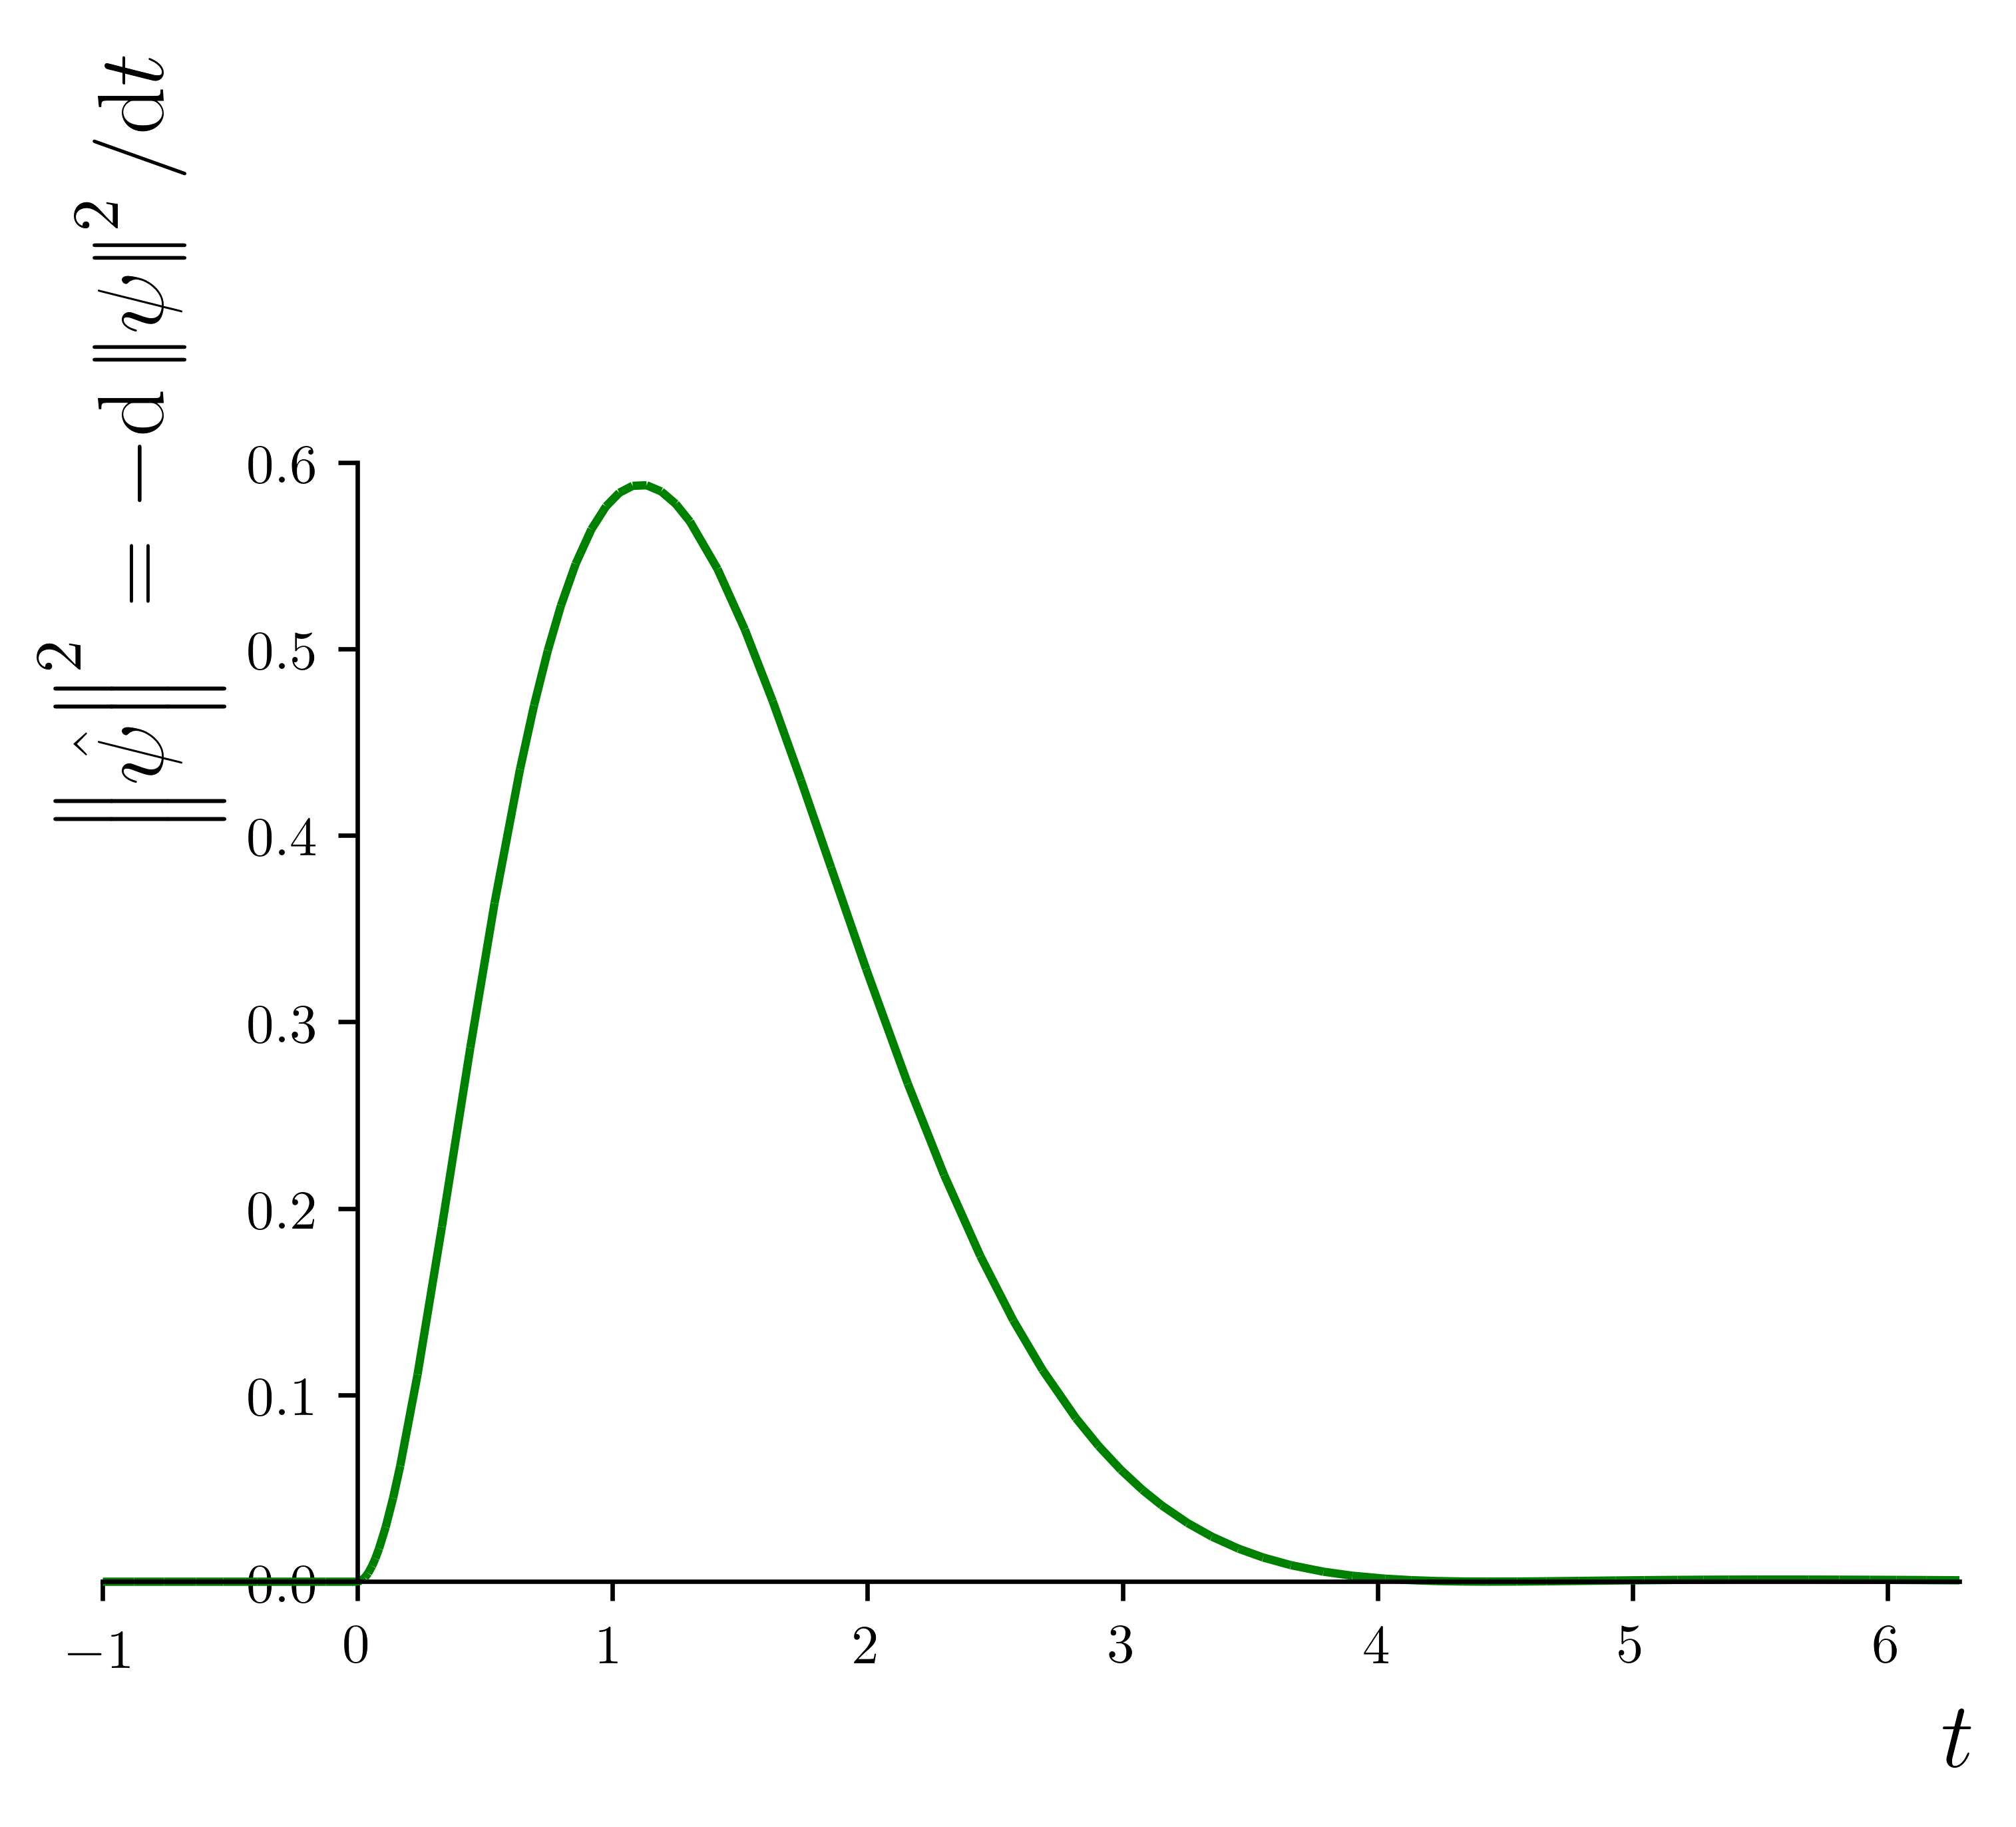
\includegraphics[width=\linewidth]{img/2ldetect/qubit_normalization_loss.png}
    \subcaption{}\label{fig:absorbed-qubit-normalization-loss:t}
  \end{subfigure}
  \begin{subfigure}[b]{0.49\textwidth}
    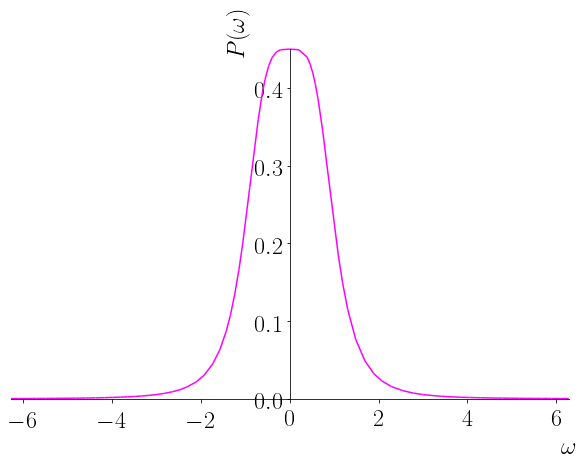
\includegraphics[width=\linewidth]{img/2ldetect/P_omega.png}
    \subcaption{}\label{fig:absorbed-qubit-normalization-loss:omega}
  \end{subfigure}
  \caption{
    Non-unitary evolution of absorbed qubit.
    \subref{fig:absorbed-qubit-normalization-loss:t}
      Detection probability in time. It's equal to the
      loss of normalization $-\dv{\norm{\psi}^2}{t}$
      (but also to the squared norm of $\hat{\psi}(t)$ as of eq. \eqref{eq:analytic:hatpsi}.
    \subref{fig:absorbed-qubit-normalization-loss:omega}
      Detection probability in the frequency domain.
  }
  \label{fig:absorbed-qubit-normalization-loss}
\end{figure}

The ``lossy'' evolution, with the two components of the qubit, is shown in Fig.~\ref{fig:absorbed-qubit-components}.
The loss of normalization $-\dv{\norm{\psi}^2}{t}$, indicating the probability of detection by absorption,
is then derived directly and shown in Fig.~\ref{fig:absorbed-qubit-normalization-loss}.

This yields the \emph{probability} of detection.
One may wonder whether it is possible to derive a corresponding \emph{probability amplitude} vector,
whose squared norm across time is equal to the said probability distribution.\footnote{
  The solution is of course not unique, but one may ask whether such functions would lead
  to quantum interference patterns and other phenomenology which may be subject of further study.
}
Within the framework of \cite{RuschhauptAbsorption}, a ``wavefunction in time'' in such sense
is the $\hat{\psi}$, as in \eqref{eq:phi_psi_kiukas}.
It is computed in detail within the
notebook in Appendix \ref{detector-model-kiukas-ruschhaupt-schmidt-werner}, eq. \eqref{eq:sympy:hatpsi},
simplifying which we obtain:
\begin{equation}\label{eq:analytic:hatpsi}
  \hat{\psi}(t) =
    i 2^{\frac{5}{4}} e^{-\frac{\sqrt{2}}{2}t}\sin(\frac{\sqrt{2}}{2}t) \theta(t)
    \ket{1}
    \text{,}
\end{equation}
with $\theta(t)$ the Heaviside step function.

\begin{remark}\label{remark:detection_area}
In general, the operator $\hat{D}$ as in \eqref{eq:schrod_complex_pot}
is such that the eigenspace corresponding to its zero eigenvalue
is the ``area'' where the detector is not sensitive. Or, in other words,
the linear span of states with zero probability of triggering the detector.
Therefore, when $\hat{D}$ (or its square root) is applied to a state vector,
for example in \eqref{eq:phi_psi_kiukas},
the components in such eigenspace are cut off and the resulting
$\hat{\psi}$, eq. \eqref{eq:analytic:hatpsi} in the example, lies at all times in the ``area of detection''
i.e. it's a multiple of $\ket{1}$ in this case.
\end{remark}

The corresponding Page--Wootters (proper) vector of $\pwspace$ is
\begin{equation}\label{eq:hatpsi:pw}
  \dket{\Phi} = \int \dd{t} \ket{t} \ox \hat{\psi}(t) \,\text{,}
\end{equation}
to which the considerations of Section \ref{sec:for-normalized-elements}
and Section \ref{sec:pure-state-approach} in terms of time--frequency
(or time--energy) uncertainty relation apply, with some analogy
to what \cite{RuschhauptAbsorption} does within its own framework
in relation to $\hat{\psi}$ and its Fourier transform.

In that regard, the \eqref{eq:hatpsi:pw} can be reformulated
\begin{equation}
  \dket{\Phi} = \int \dd{\omega} \ket{\omega} \ox \mathcal{F} \hat{\psi} (\omega) \,\text{,}
\end{equation}
where it's
\begin{equation}
  \mathcal{F} \hat{\psi} (\omega) = - \frac{\sqrt[4]{2} i}{\sqrt{\pi} \left(- \omega^{2} + \sqrt{2} i \omega + 1\right)} \ket{1}
\end{equation}
---see notebook up to eq. \eqref{eq:fhatpsi1_omega} for details.

Taking the squared modulus, a probability distribution over angular frequency
(or, equivalently, energy) is obtained:
\[
  P(\omega) = \frac{\sqrt{2}}{\pi \left(\omega^{4} + 1\right)}
  \,\text{.}
\]
See Fig. \ref{fig:absorbed-qubit-normalization-loss:omega}.